\documentclass[crop, tikz]{standalone}
\RequirePackage{luatex85}

\usetikzlibrary{
    shapes,
    positioning
}

\tikzset{component/.style={
    draw,
    rounded corners=0.1cm
}}

\tikzset{arrow/.style={->,>=stealth}}

\begin{document}
    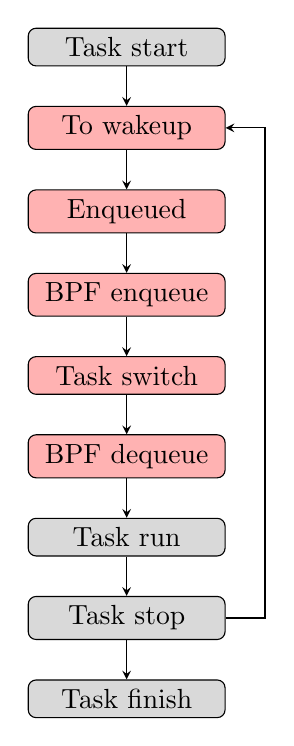
\begin{tikzpicture}[
            align=center,
            node distance=0.5cm,
            minimum width=2.5cm,
    ]
        \node[component, fill=gray!30]
            (start)
            {Task start};

        \node[component, fill=red!30, below=of start]
            (wait)
            {To wakeup};

        \node[component, fill=red!30, below=of wait]
            (enqueued)
            {Enqueued};

        \node[component, fill=red!30, below=of enqueued]
            (bpf-enqueue)
            {BPF enqueue};

        \node[component, fill=red!30, below=of bpf-enqueue]
            (task-switch)
            {Task switch};

        \node[component, fill=red!30, below=of task-switch]
            (bpf-switch-report)
            {BPF dequeue};

        \node[component, fill=gray!30, below=of bpf-switch-report]
            (task-run)
            {Task run};

        \node[component, fill=gray!30, below=of task-run]
            (task-stop)
            {Task stop};

        \node[component, fill=gray!30, below=of task-stop]
            (task-finish)
            {Task finish};

        \draw[arrow] (start) -- (wait);
        \draw[arrow] (wait) -- (enqueued);
        \draw[arrow] (enqueued) -- (bpf-enqueue);
        \draw[arrow] (bpf-enqueue) -- (task-switch);
        \draw[arrow] (task-switch) -- (bpf-switch-report);
        \draw[arrow] (bpf-switch-report) -- (task-run);
        \draw[arrow] (task-run) -- (task-stop);
        \draw[arrow] (task-stop) -- (task-finish);

        \draw[arrow] (task-stop.east) -- ++ (0.5,0) |- (wait);

    \end{tikzpicture}
\end{document}
